\documentclass[12pt]{article}
\usepackage[utf8]{inputenc}
\usepackage{bbm}
\usepackage{scrextend, layout, bm  }
\usepackage{fancyhdr,graphicx}
\usepackage[margin=1in]{geometry}
\usepackage{listings}
\pagenumbering{gobble}
\usepackage{amsmath, amssymb}
\DeclareMathOperator{\U}{\mathbb{U}}
\DeclareMathOperator{\G}{\mathbb{G}}
\DeclareMathOperator{\Tau}{\mathcal{T}}
\DeclareMathOperator{\A}{\mathcal{A}}
\DeclareMathOperator{\prob}{\mathbb{P}}
\DeclareMathOperator{\RR}{\mathbb{R}}
\DeclareMathOperator{\ind}{\mathbbm{1}}
\DeclareMathOperator{\convprob}{\stackrel{\prob}{\rightarrow}}
\DeclareMathOperator{\convw}{\stackrel{w}{\rightarrow}}
\renewcommand{\vec}[1]{\mathbf{#1}}
\usepackage{enumitem}
\pagestyle{plain}% Set page style to plain.
\setlength{\headsep}{5pt}

\begin{document}
\noindent Greg Benton, gwb67\\
CS 6241\\
Homework 1\\

\subsection*{Non-Negative Matrix Factorization}

For this homework I implemented a few non-negative matrix factorization (NMF) algorithms, namely alternating least squares (ALS), heirarchical alternating least squares (HALS), and a multiplicative update rule described in section 4 of \cite{lee2001}. Before discussing the specific algorithms, a high level overview of NMF is provided.

Non-negative matrix factorization seeks to find approximate some matrix $A \geq 0 \in \RR^{m \times n}$ with non-negative components as the product of two matrices, $W\in \RR^{m\times k}$ and $H\in \RR^{k \times n}$.  Written out, we seek $A \approx WH$, where $W, H \geq 0$ ($W$ and $H$ have all non-negative components).
The intuitive understanding is that if each row of $A$ represents one of $m$ observations of data, then matrix $W$ is composed of a $k$ dimensional vector for each data point, and $H$ is composed of coefficients that rank how important each of the $k$ dimensions is to reconstruct $A$ from it's low dimensional representative vectors in $W$.

The code for all algorithms discussed below is included at the end.

\subsubsection*{Alternating Least Squares}
Alternating least squares (ALS) is perhaps the most straightforward solution to finding $W$ and $H$ as described above, and served as a good starting point for implementing NMF. We start with some random guess for $H$ which we will denote $\hat{H}$, then solve
\[
    \hat{W} = \min_{W}||A - W\hat{H}||_{F}^{2}
\]
then
\[
    \hat{W} = \max(0, \hat{W}) \quad \text{(element-wise)}
\]
to get an estimate for $W$. This estimate, $\hat{W}$ is then plugged in to get an updated estimate for $H$,
\[
    \hat{H} = \min_{H}||A - \hat{W}H||_{F}^2
\]
then
\[
    \hat{H} = \max(0, \hat{H}) \quad \text{(element-wise)}.
\]

This is a very simple algorithm both conceptually and in implementation, but it need not converge, and there is no guarantee that the error will decrease over successive iterations of the algorithm.

\subsubsection*{Hierarchical Alternating Least Squares}
Hierarchical alternating least squares (HALS) differs from ALS in that columns of $W$ are updated one at a time, and then $H$ is updated in the same fashion as in ALS. HALS is generally a more stable algorithm and typically (under assumptions outlined in \cite{gillis2012}) converges.

Taking from \cite{gillis2012}, the columns of $W$ are updated as,
\[
    \hat{W}(:, \ell) = \max\left(0,
    \frac{XH(\ell, :)^{T} - \sum_{k\neq\ell}W(:, k)\left( H(k, :)H(\ell, :)^T \right)}
    {||H(\ell, :)||_{2}^{2}} \right).
\]
Then $\hat{W}$ is plugged in and $H$ is esimated in the same fashion as for ALS. As will be shown later this was the most effective method for the dataset chosen here.


\subsubsection*{Multiplicative Update Rule}
Lee and Seung \cite{lee2001} show that the Euclidean distance $||A - WH||$ is nonincreasing under the following update rules:
\[
    H_{ij} \leftarrow H_{ij}\frac{(W^TA)_{ij}}{(W^TWH)_{ij}}
\]
and
\[
    W_{ij} \leftarrow W_{ij}\frac{(AH^T)_{ij}}{(WHH^T)_{ij}}.
\]
This is also a somewhat simple algorithm to implement as each update is just a series of element-wise matrix operations, which is straightforward to do with a matrix library such as numpy.

\subsection*{Data}

Using the \verb|newspaper| package for python 100 of the most recent articles written on the website fivethirtyeight.com were downloaded. The articles were then labeled with their best-fitting topic of either politics, sports, science and technology, or other. This body of articles was chosen for the fact that most of the articles from FiveThirtyEight fall into a distinct category and typically they are easily identifiable (i.e. the politics articles are very distinct from those about sports). The hypothesis was that this structure should mean that separating the articles into different categories via NMF should have positive results.

Using \verb|scikit-learn| the raw text of the articles was transformed into a term frequency-inverse document frequency (tf-idf) matrix. Without delving too far into the details here, the general idea is that the entries in the tf-idf matrix, $A_{d,t}$, reflect how important term (or word) $t$ is to document (or article) $d$, scaled by how often term $j$ shows up across all articles.

More formally, we have,
\[
    A_{d, t} = tf(t, d)\times idf(t) = tf(t,d)\times (\log \frac{1 + n}{1 + df(t)} + 1)
\]
where $tf(t,d)$ is how many times term $t$ appears in document $d$, $n$ is the number of documents, and $df(t)$ is the number of documents in which term $t$ appears.

With this embedding the above algorithms were run on the dataset to project each article into a 3 dimensional space, and the results were analyzed.

\subsection*{Results}

In general the results were positive but I was initially hoping for the different topics to be more distinctly separated in their low-dimensional representation. Rather than clustering into distinct groups based on topics the articles seem to be spread along different lines in the 3 dimensional space based on topic. One thought is that given the size of the data (the full set of distinct words was about 11,000) 3 dimensions is just too few to accurately represent the articles, and that a higher dimensional representation would show more seperation between topics.

Additionally there is significant clustering near the origin, my intuition is that this is an artifact of the sparsity of the tf-idf matrix, and that the short length of some of the articles means that there is not enough information to glean a meaningful (and non-trivial) representation in such a reduced number of dimensions.

\subsubsection*{ALS}

ALS did not provide meaningful results, with the 3-D representation of the articles shown in figure \ref{als}. This could be a result of a number of different factors, but little time was spent investigating as other methods performed better.

\begin{figure}
    \centering
    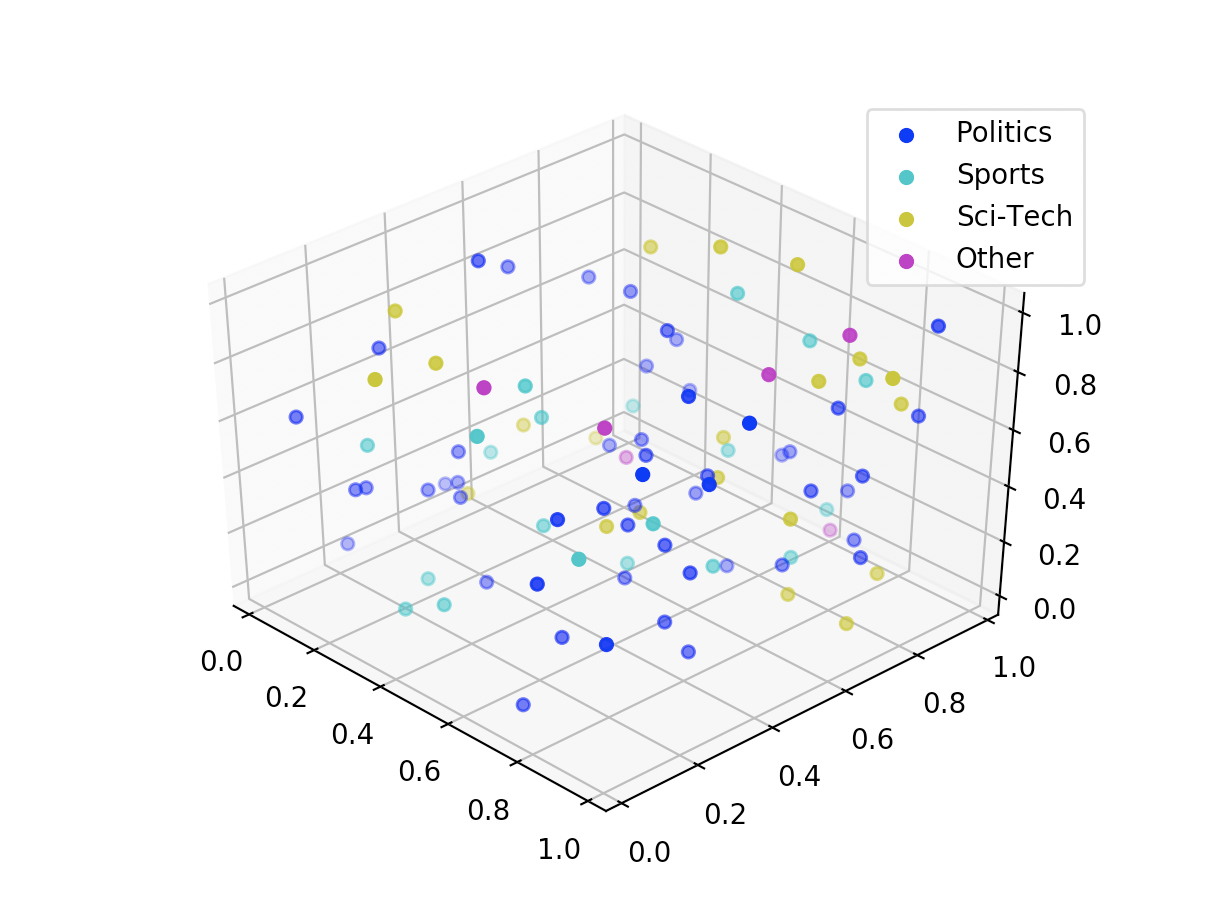
\includegraphics[scale=0.5]{als.png}
    \caption{3-D representation of 100 FiveThirtyEight articles using ALS to perform NMF.}
    \label{als}
\end{figure}


\subsubsection*{HALS}

HALS performed the best of the three algorithms implemented. The different topics did not get quite as separated spatially as initially hoped, but there is some clear dispersion between the different types of articles. It appears as though the different topics get sent out along different directions in space.
The most apparent separation is between the articles on politics and those on sports, the smaller subset of articles about science and technology see some distinct dispersion, but this is less pronounced.

It is worth noting at this point that some of the articles are really just stubs of articles; for example some of the "articles" in the dataset are just a sentence or two about the topic of a podcast, or a couple paragraphs discussing updates to the website. This may help explain some of the clustering around the origin, and why many of the `other' articles were not seperated in a meaningful way.

The result of running 100 iterations of HALS on the tf-idf matrix to project the articles into a 3-dimensional space is shown in figure \ref{hals}.

\begin{figure}
    \centering
    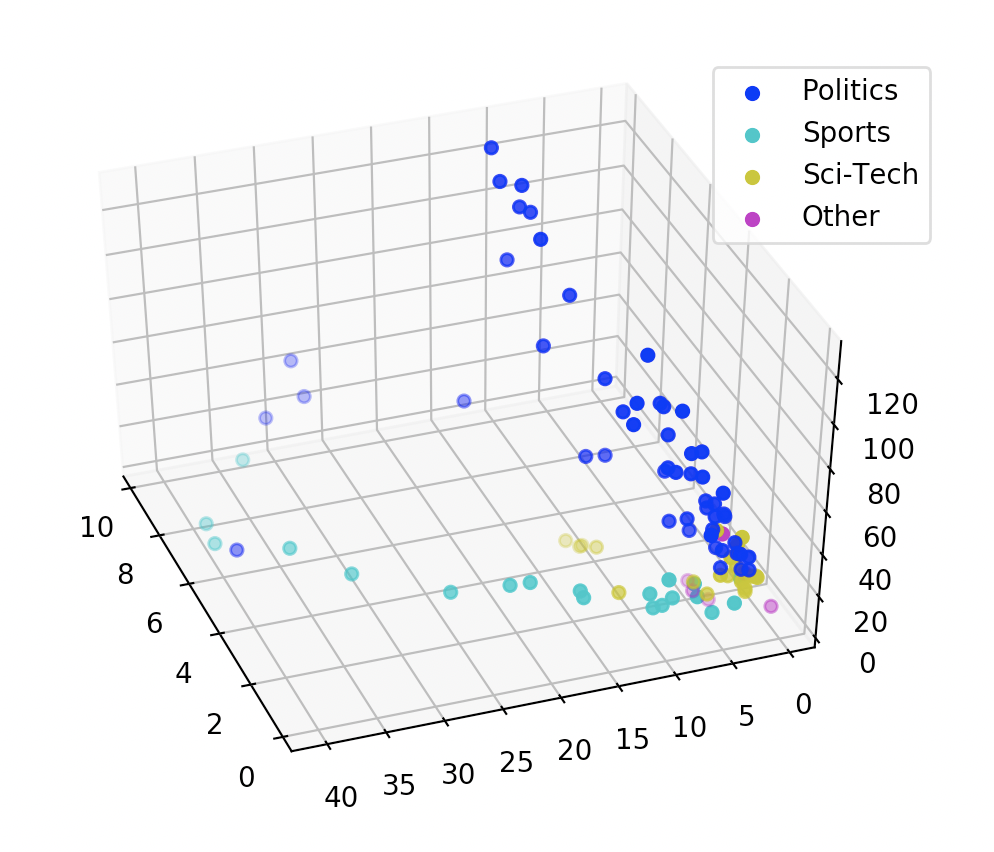
\includegraphics[scale=0.5]{hals.png}
    \caption{3-D representation of 100 FiveThrirtyEight articles using HALS to perform NMF.}
    \label{hals}
\end{figure}

\subsubsection*{Multiplicative Update Rule}

Using multiplicative update rules provides an output that is similar to HALS, but slightly less clear in the dispersion between different topics. Using multiplicative update rules the political articles seem to get sent out in two major directions while sports and science and technology get seem to be represented along the same axis (aproximately vertical from the origin).


\begin{figure}
    \centering
    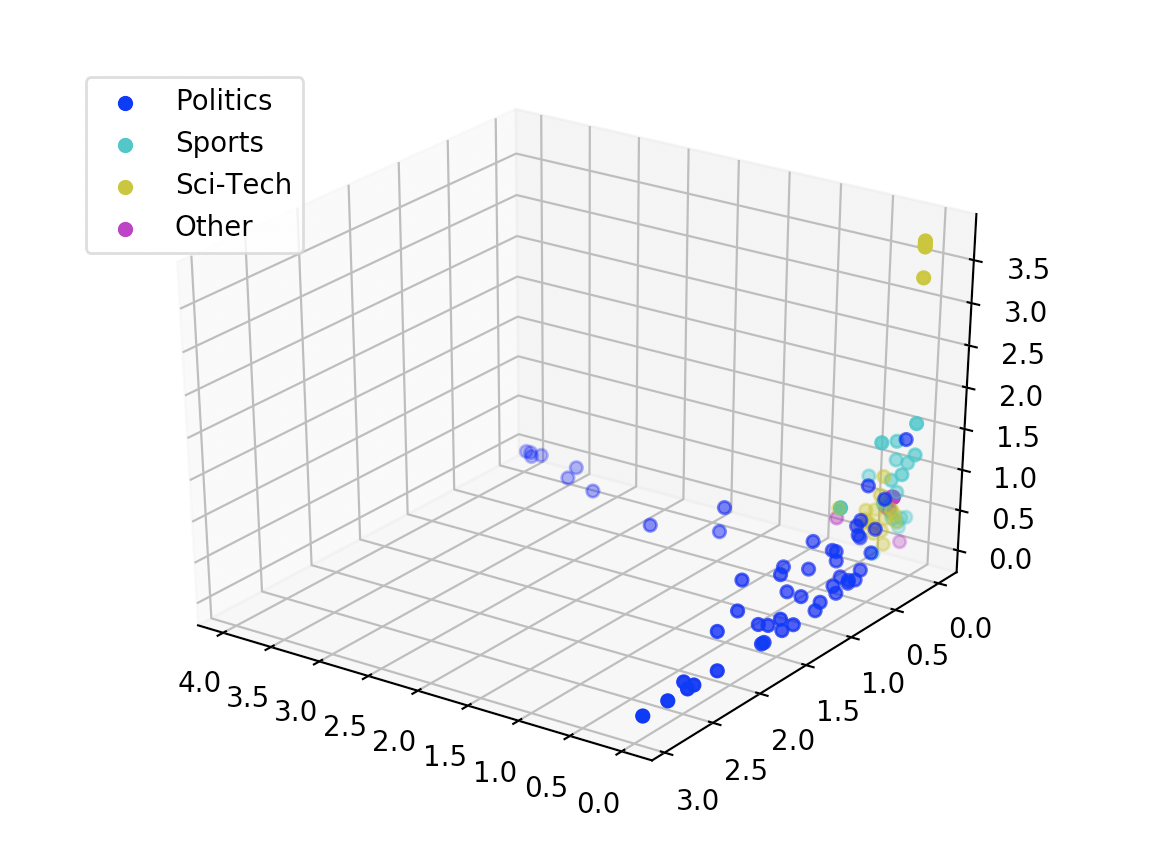
\includegraphics[scale=0.5]{mult-update.png}
    \caption{3-D representation of articles using multiplicative update rules to perform NMF.}
    \label{mult-update}
\end{figure}

\newpage
\subsection*{Code}

All raw files, data, and code can be found at \verb|https://github.com/g-benton/fivethirtyeight-topic-modeling|. The main files necessary are included in raw text below, with some files for preprocessing data omitted for the sake of brevity.

\lstset{language=Python}
\textbf{Reading In Articles}
\footnotesize
\begin{lstlisting}
import newspaper
import numpy as np
import csv
from sklearn.feature_extraction.text import TfidfTransformer, CountVectorizer
from sklearn.feature_extraction.text import TfidfVectorizer

def main():
    ## build paper and read in articles ##
    five38 = newspaper.build("http://fivethirtyeight.com/", memoize_articles=False)
    article_limit = 100
    five38_articles = five38.articles[0:article_limit]
    raw_text = [0 for art in five38_articles]
    titles = [0 for art in five38_articles]
    urls = [0 for art in five38_articles]

    ## extract raw text ##
    for ind, art in enumerate(five38_articles):
        try:
            art.download()
            art.parse()
        except:
            pass
        else:
            raw_text[ind] = art.text
            titles[ind] = art.title
            urls[ind] = art.url

    while 0 in titles:
        bad_ind = titles.index(0)
        raw_text.pop(bad_ind)
        titles.pop(bad_ind)

    fpath = "/Users/greg/Google Drive/Spring 19/CS6241/fivethirtyeight-topic-modeling/extract-data/"
    fname = "five38_data.csv"
    with open(fpath + fname, "w", newline='') as f:
        writer = csv.writer(f)
        writer.writerow(raw_text)
        writer.writerow(titles)
        writer.writerow(urls)

    ## one stop shop to do tf-idf transform ##
    vectorizer = TfidfVectorizer(stop_words='english')
    X = vectorizer.fit_transform(raw_text)
    X = X.toarray()
    fname = 'five38_tfidf'
    np.save(file=fpath+fname, arr=X)

    return 1

if __name__ == '__main__':
    main()
\end{lstlisting}

\textbf{ALS Script}
\begin{lstlisting}
import numpy as np
from scipy.sparse import random as sciRand
from scipy.optimize import nnls
from mpl_toolkits.mplot3d import Axes3D
import math
import csv
import sys
sys.path.append("/Users/greg/Google Drive/Spring 19/CS6241/fivethirtyeight-topic-modeling/extract-data/")
import matplotlib.pyplot as plt

def update_W(X, W, H, rank=3):
    Wt = np.linalg.lstsq(np.transpose(H), np.transpose(X), rcond=None)
    return W

def update_H(X, W):
    H = np.linalg.lstsq(W, X, rcond=None)[0]
    H[H < 0] = 0
    return H

def ALS(X, rank=3, n_iters=100, seed=66):
    np.random.seed(seed)
    x_norm = np.linalg.norm(X)
    n = X.shape[0]
    m = X.shape[1]
    W = np.random.rand(n, rank)
    H = np.random.rand(rank, m)

    # n_iters = 50
    errors = [None for ii in range(n_iters)]
    for iter in range(n_iters):
        W = update_W(X, W, H, rank)
        H = update_H(X, W)
        errors[iter] = np.divide(np.linalg.norm(X - np.dot(W, H)), x_norm)

    return W, H, errors
\end{lstlisting}

\textbf{HALS Script}
\begin{lstlisting}
import numpy as np
from scipy.sparse import random as sciRand
from scipy.optimize import nnls
from mpl_toolkits.mplot3d import Axes3D
from matplotlib.lines import Line2D
import math
import csv
import sys
sys.path.append("/Users/greg/Google Drive/Spring 19/CS6241/fivethirtyeight-topic-modeling/extract-data/")
import matplotlib.pyplot as plt

def update_W(X, W, H, rank=3):
    ## update column by column ##
    for col in range(rank):

        offset = np.zeros_like(W[:, col])
        for kk in range(rank):
            if kk != col:
                offset += np.dot(W[:, kk], np.dot(H[kk ,:], np.transpose(H[col, :])))


        new_vec = np.divide(np.dot(X, H[col, :]) + offset, np.linalg.norm(H[:, col]))
        new_vec[new_vec < 0] = 0
        W[:, col] = new_vec
        ## NOTE: This method uses previous updates to compute next iterates,
        ## may want to change this if there are convergence issues.
    return W

def update_H(X, W):
    H = np.linalg.lstsq(W, X, rcond=None)[0]
    H[H < 0] = 0
    return H

def HALS(X, rank=3, n_iters=100, seed=66):
    x_norm = np.linalg.norm(X)
    n = X.shape[0]
    m = X.shape[1]
    np.random.seed(seed)
    W = np.random.rand(n, rank)
    H = np.random.rand(rank, m)

    errors = [None for ii in range(n_iters)]
    for iter in range(n_iters):
        W = update_W(X, W, H, rank)
        H = update_H(X, W)
        errors[iter] = np.divide(np.linalg.norm(X - np.dot(W, H)), x_norm)

    return W, H, errors
\end{lstlisting}

\textbf{Multiplicative Update Script}
\begin{lstlisting}
import numpy as np
from scipy.sparse import random as sciRand
from scipy.optimize import nnls
from mpl_toolkits.mplot3d import Axes3D
from matplotlib.lines import Line2D
import math
import csv
import sys
sys.path.append("/Users/greg/Google Drive/Spring 19/CS6241/fivethirtyeight-topic-modeling/extract-data/")
import matplotlib.pyplot as plt

def update_H(X, W, H):
    numer = np.dot(np.transpose(W), X)
    denom = np.dot(np.dot(np.transpose(W), W), H)
    H = np.multiply(H, np.divide(numer, denom))
    # H[H<0] = 0

    return H

def update_W(X, W, H):
    numer = np.dot(X, np.transpose(H))
    denom = np.dot(np.dot(W, H), np.transpose(H))
    W = np.multiply(W, np.divide(numer, denom))
    # W[W<0] = 0

    return W

def mult_update(X, rank=3, n_iters=100, seed=66):
    x_norm = np.linalg.norm(X)
    n = X.shape[0]
    m = X.shape[1]
    np.random.seed(seed)
    W = np.random.rand(n, rank)
    H = np.random.rand(rank, m)

    errors = [None for ii in range(n_iters)]
    for iter in range(n_iters):
        H = update_H(X, W, H)
        W = update_W(X, W, H)
        errors[iter] = np.divide(np.linalg.norm(X - np.dot(W, H)), x_norm)

    return W, H, errors
\end{lstlisting}

\textbf{Plotting Script}
\begin{lstlisting}
import matplotlib.pyplot as plt
from mpl_toolkits.mplot3d import Axes3D
from matplotlib.lines import Line2D

def plotting(W, classes, labels=['Politics', 'Sports', 'Sci-Tech', 'Other']):
    plt_colors = ['b', 'c', 'y', 'm']
    n_cls = 4

    fig = plt.figure()
    ax = fig.add_subplot(111, projection='3d')

    plt_inds = [0 for i in range(n_cls)]
    for cls in range(n_cls):
        plt_inds[cls] = [i for i, c in enumerate(classes) if int(c)==cls]
        # print(plt_inds[cls])
        ax.scatter(xs=W[plt_inds[cls], 0], ys=W[plt_inds[cls], 1],
            zs=W[plt_inds[cls],2], c=plt_colors[cls], label=labels[cls])

    ax.legend()
    plt.show()

    return 1
\end{lstlisting}

\textbf{Main Runner Script}
\begin{lstlisting}
import sys
import csv
import numpy as np

sys.path.append("/Users/greg/Google Drive/Spring 19/CS6241/fivethirtyeight-topic-modeling/nmf-files/")
from HALS import *
sys.path.append("/Users/greg/Google Drive/Spring 19/CS6241/fivethirtyeight-topic-modeling/main-files/")
# sys.path.append("./nmf-files/")
# sys.path.append("./main-files/")
# sys.path.append("./extract-data/")
from plotting import plotting

def main():
    fpath = "/Users/greg/Google Drive/Spring 19/CS6241/fivethirtyeight-topic-modeling/extract-data/"
    fname = "five38_data.csv"
    with open(fpath + fname, newline='') as f:
        reader = csv.reader(f)
        raw_dat = list(reader)

    raw_text = raw_dat[0]
    titles = raw_dat[1]
    classes = raw_dat[2]

    fname = "five38_tfidf.npy"
    X = np.load(fpath + fname)

    W, H, errs = HALS(X, n_iters=100, rank=3,seed=21)
    plotting(W, classes=classes)

if __name__ == '__main__':
    main()
\end{lstlisting}
\newpage
\nocite{*}
\bibliography{main}
\bibliographystyle{plain}

\end{document}
